\chapter{Implementierung}

Im Folgenden wird vorgestellt, wie das beschriebene Verfahren, welches wir auf Basis der vorigen
\"Uberlegungen erhalten haben, konkret in Programmcode umgesetzt wird. Aufgrund des hohen Ma{\ss}es an Kontrolle \"uber den Einsatz der
Hardware, des damit einhergehenden Geschwindigkeitsvorteils, sowie der erleichterten Anbindung an bestehende Frameworks, wurde zu
diesem Zweck die Programmiersprache C++ gew\"ahlt. Der funktionale Kern des Programms wird hierbei als \textit{statische Bibliothek}
realisiert, diese kann dann zum konkreten Einsatz bequem eingebunden werden.

\section{Aufbau der Software}

Das Gesamtger\"ust des Programms wurde auf dem Paradigma der \textit{objektorientierten Programmierung} aufgebaut. Dies bedeutet,
dass der Algorithmus
und die zugrundeliegende Funktionalit\"at in Klassen gekapselt und dem Benutzer durch klar definierte Schnittstellen zug\"anglich
gemacht wird.

\subsection{Klassendesign}

\fref{fig:klassen} gibt einen \"Uberblick \"uber die Struktur der wichtigsten Klassen und Interfaces in Form eines UML-Klassendiagramms.
Weniger wichtige Beziehungen und Operationen, sowie Klassen, die nur der reinen Repr\"asentation von Daten dienen, wurden bewusst
aus Gr\"unden der \"Ubersichtlichkeit ausgespart.
Die konkreten Aufgaben aller Klassen werden im Folgenden n\"aher beschrieben.

\begin{figure}
  \label{fig:klassen}
  \centering
  \begin{tikzpicture}%[show background grid]
    \begin{class}[text width=15cm]{Propagator}{0,0}
      \attribute{- fieldDescriptor: FieldDescriptor}

      \operation{+ Propagator( fieldDescriptor: FieldDescriptor )}
      \operation{+ getTrack( particle: Particle, stoppingCondition: Condition, initialTimeStep: double ): vector<Particle>}
    \end{class}

    \begin{interface}[text width=7.5cm]{FieldDescriptor}{-4, -4}
      \operation[0]{getStrength( location: Vector3D ): Vector3D}
    \end{interface}
    
    \begin{interface}[text width=6.5cm]{Condition}{4, -4}
      \operation[0]{check( track: vector<Particle> ): bool}
    \end{interface}

    \begin{class}[text width=6cm]{MaximumDistanceCondition}{-4, -7}
      \implement{Condition}
      \attribute{- maxDistance: double}
      \attribute{- referencePoint: Vector3D}
    \end{class}

    \begin{class}[text width=6cm]{PlaneIntersectionCondition}{4, -7}
      \implement{Condition}
      \attribute{- plane: Plane3D}
    \end{class}

    \draw[umlcd  style  dashed  line ,->] (Propagator) --node[above , sloped ,
      black]{} (FieldDescriptor);

    \draw[umlcd  style  dashed  line ,->] (Propagator) --node[above , sloped ,
      black]{} (Condition);
  \end{tikzpicture}
  \caption{Die strukturelle Anordnung der wichtigsten Klassen und Schnittstellen.}
\end{figure}

\paragraph{Particle}

Enth\"alt Informationen \"uber den Zustand eines Teilchens. Hierzu z\"ahlen die Eigenschaften \textit{Zeit, Energie, Masse, Ladung,
  Ort} und \textit{Impuls}. Die Geschwindigkeit des Teilchens kann unter Kenntnis der Masse mithilfe des Impulses bestimmt werden.

\paragraph{Vector3D}
Wird verwendet, um Vektoren im dreidimensionalen Raum darzustellen. Implementiert au{\ss}erdem diverse Vektoroperationen wie
\textit{Skalarmultiplikation, Vektoraddition} oder das \textit{Skalarprodukt}. Die Rotation eines Vektors, welche in der
Transformation zur Anwendung kommt, ist ebenfalls innerhalb dieser Klasse realisiert worden.

\paragraph{Plane3D}
Repr\"asentiert eine Ebene im dreidimensionalen Raum. Hierzu wird der Normalenvektor, sowie ein beliebiger Punkt in der Ebene
gespeichert.

\paragraph{FieldDescriptor}
Definiert eine Schnittstelle, welche spezifiziert, wie auf die Informationen eines magnetischen Feldes zugegriffen werden kann.
Durch Angabe des gew\"unschten Ortes, an welchem die Feldst\"arke bestimmt werden soll, kann diese erfragt werden.

\paragraph{Condition}
Liefert eine Schnittstelle f\"ur Abbruchbedingungen. Die implementierenden Klassen erhalten in der Methode \textit{check} eine
Referenz auf die bis dahin vorliegende Flugbahn. Soll das Verfahren abgebrochen werden, wird der Wert \textit{true} zur\"uckgegeben.

\paragraph{MaximumDistanceCondition}
Konkrete Implementierung der \textit{Condition}-Schnittstelle. Gibt den Wahrheitswert \textit{true} zur\"uck, sobald eine maximale
Distanz zu einem Referenzpunkt \"uberbr\"uckt wurde.

\paragraph{PlaneIntersectionCondition}
Diese Implementierung der \textit{Condition}-Schnittstelle gibt den Wert \textit{true} zur\"uck, sobald die Flugbahn eine
gegebene Ebene schneidet.

\paragraph{Propagator}
Kapselt den beschriebenen Algorithmus zur Bestimmung der Teilchenflugbahn. Bei der Erzeugung des Propagators muss ein
\textit{FieldDescriptor} angegeben werden, welcher das magnetische Feld beschreibt, auf welchem die Simulation durchgef\"uhrt werden
soll. Die Methode \textit{getTrack} enth\"alt im Wesentlichen den bereits vorgestellten Pseudocode und gibt
die Flugbahn als Aneinanderreihung von Teilchenzust\"anden zur\"uck.

\subsection{M\"oglichkeit der Einbindung}

Um die Software nun einbinden und nutzen zu k\"onnen, muss zun\"achst die Datei \textit{libpropagator.a} dem \textit{Linking-Prozess}
hinzugef\"ugt werden. Die Bibliotheksdatei erh\"alt man direkt aus der \"Ubersetzung, welche wie in \fref{sec:cmake} beschrieben
durch den Aufruf der Programme \textit{CMake} und \textit{Make} (Auf UNIX-Betriebssystemen) erfolgt. Weiterhin m\"ussen die
mitgelieferten \textit{Header-Dateien} in einem Ordner liegen, der dem Compiler bekannt ist.

Bei der Nutzung des Verfahrens muss zun\"achst das magnetische Feld zugreifbar gemacht werden, auf welchem simuliert werden soll.
Hierzu kann bequem das Interface \textit{FieldDescriptor} erweitert werden. Im n\"achsten Schritt l\"asst sich unter Zuhilfenahme
dieser neu
erstellten Klasse ein Objekt vom Typ \textit{Propagator} instanziieren. Um die Methode \textit{getTrack} ausf\"uhren zu k\"onnen,
welche die gew\"unschten Ergebnisse liefert, muss zun\"achst ein Objekt vom Typ \textit{Particle} erzeugt werden. Dieses
repr\"asentiert den Startzustand des Teilchens in der Simulation. Anschlie{\ss}end muss man eine Abbruchbedingung ausw\"ahlen,
ist man mit den beiden bestehenden Bedingungen noch nicht zufrieden, l\"asst sich das Interface \textit{Condition} nach beliebigen
W\"unschen erweitern. Je nach erforderlicher Genauigkeit muss nun der Parameter \textit{initialTimeStep} angepasst werden, schon
l\"asst sich die Simulation starten.

\section{Verwendete Entwicklerwerkzeuge}

Im Zuge der Erstellung der Simulationssoftware wurden einige Werkzeuge eingesetzt, die den Entwicklungsprozess besonders im Hinblick
auf das \"Ubersetzen und Testen der Programmteile wesentlich unterst\"utzt und vereinfacht haben.
Diese werden im Folgenden kurz beschrieben.

\subsection{CMake}
\label{sec:cmake}

Das plattformunabh\"angige Programmierwerkzeug CMake \textit{(cross platform make)} wurde verwendet, um einen komplikationslosen
Build-Prozess zu gew\"ahrleisten. CMake verf\"ugt \"uber die F\"ahigkeit, automatisch Abh\"angigkeiten zwischen den verschiedenen
Quelldateien zu erkennen. Zusammen mit den weiteren Instruktionen, wie das gegebene Projekt zu \"ubersetzen ist, werden diese
Abh\"angigkeiten in ein resultierendes \textit{Makefile} \"uberf\"uhrt, welches die Basis f\"ur das unter UNIX verf\"ugbare
Build-Management-Tool \textit{Make} bildet, mit dessen Hilfe das Programm anschlie{\ss}end reibungslos \"ubersetzt werden kann.
Arbeitet man auf einer anderen Plattform als UNIX, beispielsweise auf Windows, l\"asst sich mit
CMake auch ohne Probleme ein \textit{Visual Studio}-Projekt erzeugen. Somit kann das Programm plattformunabh\"angig \"ubersetzt und
eingesetzt werden.

Ein weiterer Vorteil von CMake besteht darin, einzelne Komponenten der Software unabh\"angig zu verarbeiten. In diesem Fall wurde
es durch CMake beispielsweise m\"oglich, die Test- und Demonstrationsf\"alle als eigenst\"andige ausf\"uhrbare Programme zu
\"ubersetzen. Diese Programme betten allesamt die Kernbibliothek \textit{libpropagator.a} ein, was die lose und bequeme Kopplung
von funktionalem Programmkern und speziellem Anwendungsfall verdeutlicht.

\subsection{Google Test}

Um die Korrektheit der einzelnen Programmteile zu gew\"ahrleisten, mussten zahlreiche Testf\"alle kodiert werden. Hierbei wurde
nach dem Unittest-Prinzip vorgegangen, welches es erm\"oglicht, Testf\"alle f\"ur unabh\"angige Komponenten unabh\"angig voneinander
zu betrachten. Auf diese Weise konnte zum Beispiel das Berechnen der Drehwinkel getrennt von der tats\"achlichen Transformation
untersucht werden. Durch diese feingranulare Spezifikation der Testf\"alle k\"onnen Fehler schnell identifiziert, zugeordnet
und damit auch schnell behoben werden.

Eine Programmbibliothek, welche diese Art der Arbeitsweise bestens unterst\"utzt, wird von der Firma Google unter dem Namen
\textit{Google Test}
oder auch \textit{GTest} bereitgestellt. GTest erm\"oglicht es, eine Reihe einzelner Unit-Tests zu kodieren und diese komfortabel
hintereinander auszuf\"uhren. Dieses Verhalten erleichtert die Durchf\"uhrung von sogenannten \textit{Regressionstests} ungemein:
Sobald eine \"Anderung am Programm vorgenommen wurde, k\"onnen im Anschluss alle Testf\"alle bequem durch einen Aufruf von GTest
ausgef\"uhrt werden. So l\"asst sich leicht erkennen, ob die eingef\"uhrte  \"Anderung die Korrektheit des Programms weiterhin
gew\"ahrleistet.

\section{Visualisierung und Demonstration}

Um die Ergebnisse der Simulationen f\"ur einzelne Beispiele zu veranschaulichen, wurde das Programm \textit{gnuplot} eingesetzt.
Die jeweiligen Positionen, die das Teilchen auf seinem Weg durch das Magnetfeld einnimmt, werden durch Punkte repr\"asentiert,
welche durch Linien miteinander verbunden sind. Eine Auswahl an konkreten Demonstrationen wird im Folgenden vorgestellt.

\subsection{Schraubenlinien im homogenen Magnetfeld}

Der einfachste Fall einer Demonstration bel\"auft sich auf ein rein homogenes Magnetfeld. Wie in \fref{fig:homogeneous_plot} zu sehen,
ergeben sich hier genau die Schraubenlinien, welche bereits zu Anfang dieser Arbeit beschrieben wurden.

\begin{figure}[h]
  \label{fig:homogeneous_plot}
  \centering
  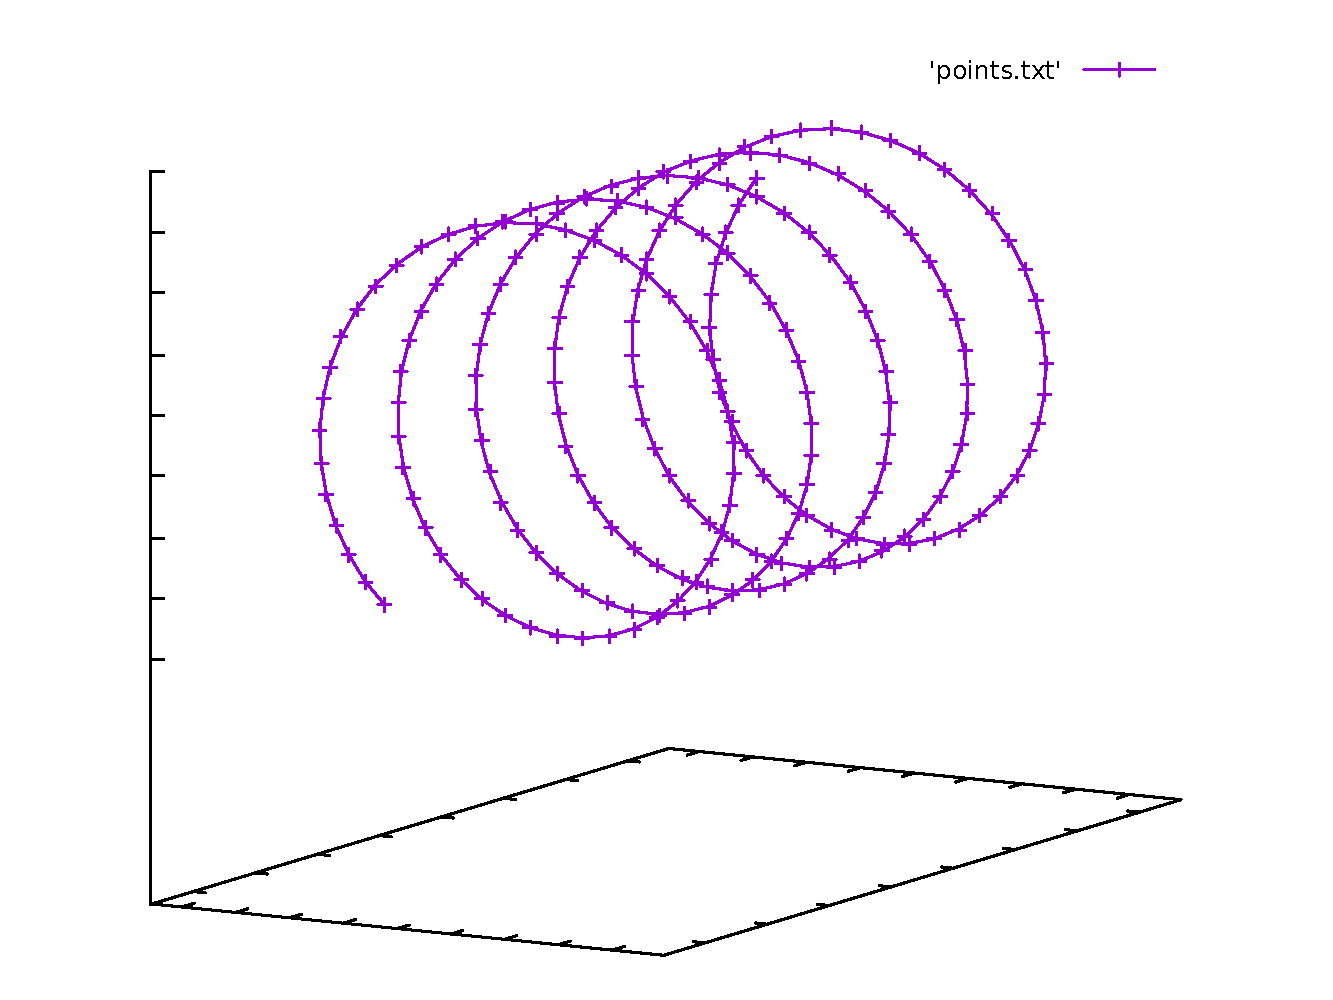
\includegraphics[width=0.75\textwidth]{gnuplot/homogeneous}
  \caption{Die Schraubenlinien der Teilchenbewegung im homogenen Magnetfeld.}
\end{figure}

\subsection{Abbruchbedingung bei Schnitt mit Ebene}

Der Fall, dass die Simulation beendet werden soll, sobald das Teilchen eine Ebene durchquert, sei hier dargestellt. Wie in
\fref{fig:stop_plane} zu sehen ist, vollzieht das Teilchen zun\"achst seine charakteristische Bewegung und trifft anschlie{\ss}end
auf eine Ebene. Dies l\"ost die bereits beschriebene \textit{PlaneIntersectionCondition} aus, was das Ende der Simulation zur Folge
hat.

\begin{figure}[h]
  \label{fig:stop_plane}
  \centering
  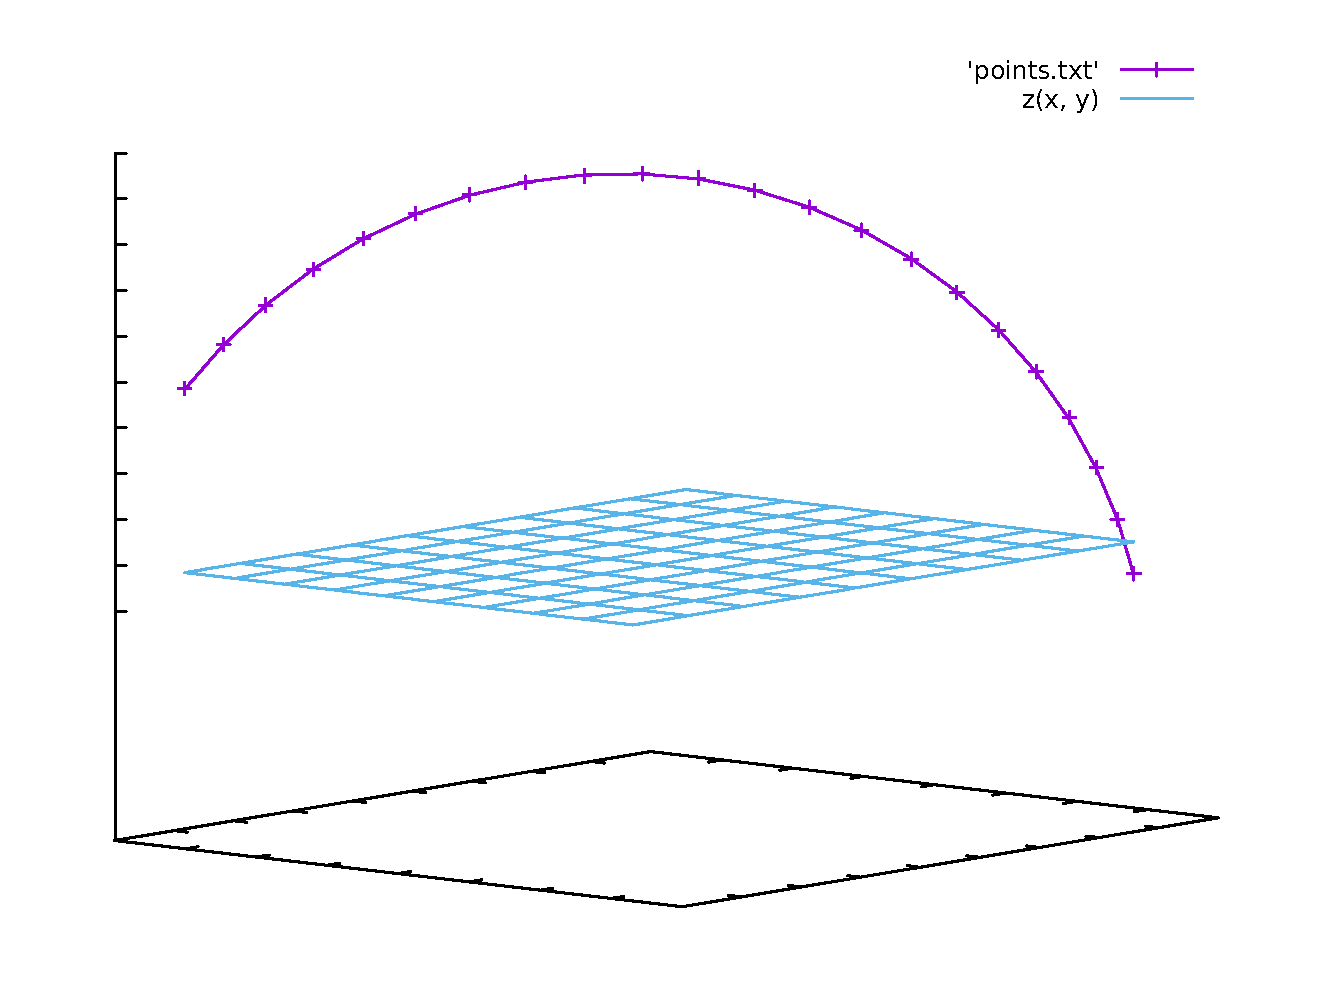
\includegraphics[width=0.75\textwidth]{gnuplot/stop_plane}
  \caption{Die Simulation wird beendet, sobald das Teilchen die Ebene durchquert.}
\end{figure}

\subsection{Abrupter \"Ubergang zwischen zwei homogenen Magnetfeldern}

Um zu demonstrieren, wie sich das Verfahren bei inhomogenen Magnetfeldern verh\"alt, wird in diesem Beispiel der unmittelbare
\"Ubergang zwischen zwei homogenen Magnetfeldern simuliert. Das zweite Feld zeigt hierbei genau in die entgegengesetzte Richtung
des ersten Feldes. Wie in \fref{fig:two_fields} zu sehen, f\"uhrt dieser \"Ubergang wie erwartet zu einer Umkehrung der
Kreisbewegung. Die gleichf\"ormige Komponente der Bewegung bleibt hiervon unbeeinflusst.

\begin{figure}[h]
  \label{fig:two_fields}
  \centering
  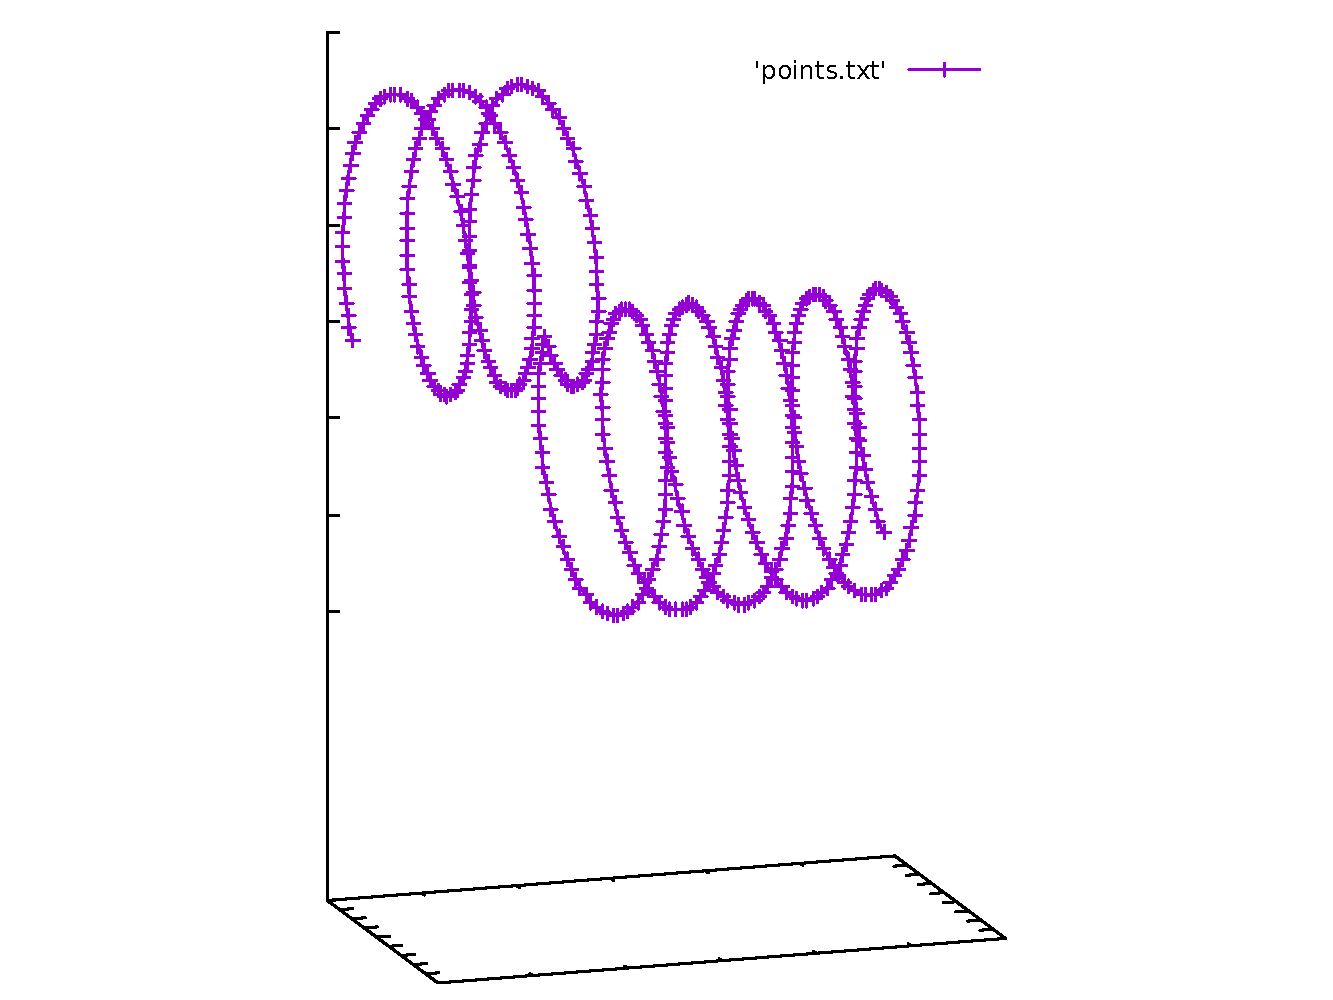
\includegraphics[width=0.75\textwidth]{gnuplot/two_fields}
  \caption{Der abrupte \"Ubergang zwischen den Feldern resultiert in einer Umkehrung der Kreisbewegung.}
\end{figure}
